\documentclass[aspectratio=169, compress, table]{beamer}

\usepackage{forest}
\usepackage{amsmath}
\usepackage{tabularx}

\usepackage{svg}
\usepackage{beamercolorthemelmu}
\usepackage[utf8]{inputenc}
\usepackage{array}
\usepackage{booktabs}
\usepackage{multirow}
\usepackage{tabularx}
\usepackage{array,xcolor}
\usepackage{dsfont}
\usepackage[normalem]{ulem}
\usepackage{listings}
\usepackage{tikz}
\usetikzlibrary{calc,patterns,petri}
\usepackage{pifont}
\usepackage[noend]{algpseudocode}
\usepackage[normalem]{ulem}
\usepackage{subfiles}
\usepackage{import}
% align oversets (available in TeXLive 18 - overleaf currently runs w/ texlive 17 - 5.11.19)
% \usepackage{aligned-overset}
\usepackage{bbm}

% Sfehs personal commands (the same as in dbstmpl.sty)
\newcommand{\plforest}[1]{{\begin{forest}   for tree={child anchor=north, rounded corners,align=center,draw=black!100,fill=blue!20},   terminal/.style={rectangle,},   fixnode/.style={fill=blue!60,},   observation/.style={rectangle,},   variable/.style={rectangle,},  samenode/.style={fill=blue!40,},  newnode/.style={fill=green!60,}, changenode/.style={fill=orange!60,},   nodeinsert/.style={fill=green!50,},   nodechanged/.style={fill=orange!50,}, #1 \end{forest}}}
\newcommand{\rsymp}{\xrightarrow{\text{simplify}}}

% Indicate clickability by colour
\hypersetup{
	colorlinks,
	urlcolor=blue,
	linkcolor=black,
%	citecolor={blue!50!black},
%	urlcolor={blue!70!black}
	bookmarksdepth=5,
}

% Set color theme
\usecolortheme{lmu}
% Set outer theme (~layout)
\useoutertheme{dbsthesis}

\AtBeginSection[]{%
	\begin{frame}[plain, squeeze, noframenumbering]{Outline}%
		\small%
		\setcounter{tocdepth}{5}%
		\begin{columns}[t]%
			\begin{column}{.8\textwidth}%
				\tableofcontents[
				currentsection,
				currentsubsection,
				subsectionstyle=show/shaded/hide,
				subsubsectionstyle=show/show/hide,
				sections=1-
				]%
			\end{column}%
			\hfill
		\end{columns}%
	\end{frame}%
}
% Set metadata
\author{Simon Fehrer}
\title[
    \textcolor{white}{Creating familiar Reinforcement Learning Policies with Genetic Programming}]
    {Creating familiar Reinforcement Learning Policies with Genetic Programming}
\newcommand{\inserthesistype}{Master Thesis}
\institute[DBS]{Ludwig-Maximilians-Universität München\\Lehrstuhl für Datenbanksysteme und Data Mining}
\newcommand{\insertsupervisor}{Prof. Dr. Volker Tresp}
\newcommand{\insertadvisor}{Dr. Michel Tokic, Dr. Steffen Udluft, Dr. Daniel Hein}
\date{\today}

% Custom macros
% IMPORTANT: Use \input to avoid excluding macros definitions when working on a single chapter
% Math
\newcommand{\RR}{\mathbb{R}}
\newcommand{\NN}{\mathbb{N}}

% Checkmark and cross symbols
\newcommand{\cmark}{\textcolor{beamer@lmu_green}{\ding{51}}}
\newcommand{\xmark}{\textcolor{red}{\ding{55}}}

% Footnote without marker
\newcommand\blfootnote[1]{%
  \begingroup
  \renewcommand\thefootnote{}\footnote{#1}%
  \addtocounter{footnote}{-1}%
  \endgroup
}

% Argmin/argmax
\DeclareMathOperator*{\argmin}{argmin}
\DeclareMathOperator*{\argmax}{argmax}

% Multi-line statements in algorithmic with correct indendation
\makeatletter
\newcommand{\multiline}[1]{%
  \begin{tabularx}{\dimexpr\linewidth-\ALG@thistlm}[t]{@{}X@{}}
    #1
  \end{tabularx}
}
\makeatother

\begin{document}

\begin{frame}[plain, noframenumbering]
\titlepage
\end{frame}










\section{Outline} %%%%%%%%%%%%%%%%%%%%%%%%%%%%%%%%%%%%%%%%%%%%%%%%%%%%%%%%%%%%%%%%%%%%%%%%%%%%%%%%%%%

\begin{frame}{Outline}
%
\includegraphics[height=0.89\textheight]{img/concept.png}  % aka 76mm
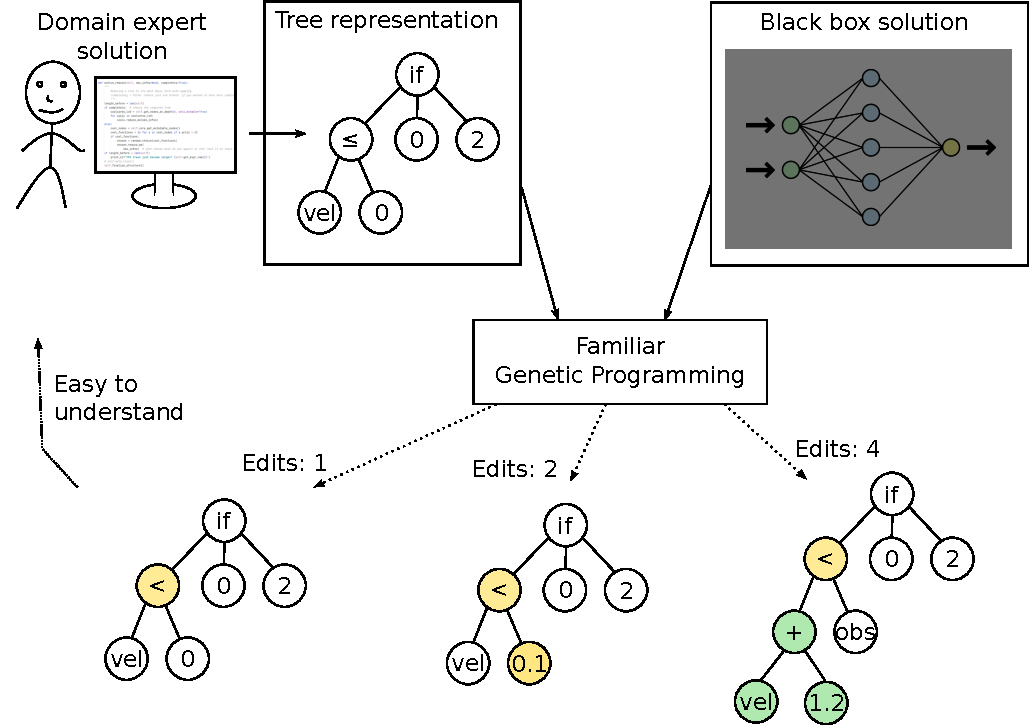
\includegraphics[height=0.89\textheight]{../img/inkscape/concept.pdf}
\end{frame}


\begin{frame}{Extending an Expert Program}
\centering
\includegraphics[height=0.85\textheight]{img/genetic_extensions.pdf} 
\end{frame}








\section{Reinforcement Learning} %%%%%%%%%%%%%%%%%%%%%%%%%%%%%%%%%%%%%%%%%%%%%%%%%%%%%%%%%%%%%%%%%%%%%%%%%%%%%%%%%%%

\begin{frame}{Reinforcement Learning}
\centering

\includegraphics[height=0.6\textheight]{img/agent-env.png} 
\end{frame}


\begin{frame}{Mountain Car Benchmark}
 \begin{table}[th]
 \begin{centering}
 \begin{tabular}{cccc}
 \multirow{6}{*}{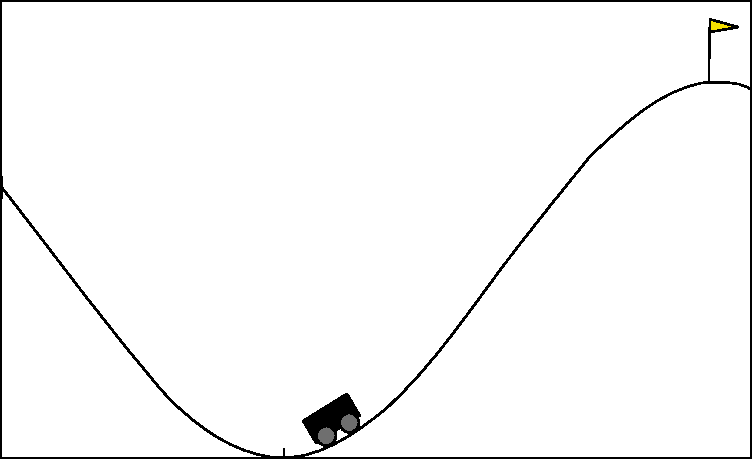
\includegraphics[width=5cm]{../img/inkscape/mountaincar_dummy}} &  & \multicolumn{2}{c}{Observation space}\tabularnewline
 \cline{3-4} \cline{4-4} 
  &  & position & $[-1.2, 0.6]$\tabularnewline
  &  & velocity & $[-0.07, 0.07]$\tabularnewline
 \cline{3-4} \cline{4-4} 
  &  &  & \tabularnewline
  &  & \multicolumn{2}{c}{action space}\tabularnewline
 \cline{3-4} \cline{4-4} 
  &  & push & \{left, none, right\}\tabularnewline
 %workaround latex pdf format idk why &  &  & \tabularnewline
 \end{tabular}
 \par\end{centering}
% \caption{The main features of the Mountain car problem. The position of the car is by a factor of 10 larger than the speed. \label{mountaincar-overview}}
\end{table}
\end{frame}


\begin{frame}{Industrial Benchmark}
   \begin{itemize}
 	  \item Represents an industrial process
 	  \item 
 	  \item 
   \end{itemize}
 \begin{table}[tph]
 \begin{tabular}{lcc}
  \toprule 
  & MC & IB\tabularnewline
  \midrule
  Observables & 2 & 6\tabularnewline
  Action dimensions & 1 & 3\tabularnewline
  Reward & discrete & continuous\tabularnewline
  Episode end & at target / 200 & none\tabularnewline
  Stochasticity & none & state-dependent\tabularnewline
  Observable & fully & partially\tabularnewline
  \bottomrule
 \end{tabular}
\caption{\label{tab:mc-ib-comparisson}A comparison of the benchmarks used.}
\end{table}
\end{frame}






\section{Genetic Programming} %%%%%%%%%%%%%%%%%%%%%%%%%%%%%%%%%%%%%%%%%%%%%%%%%%%%%%%%%%%%%%%%%%%%%%%%%%%%%%%%%%%

\begin{frame}{Interpretability of Formulae}
 \centering
 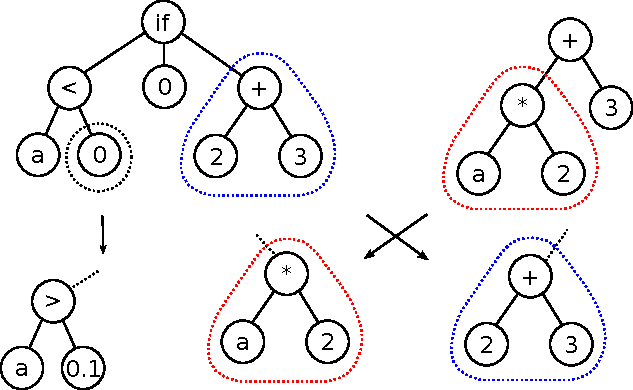
\includegraphics[height=0.75\textheight]{../img/inkscape/GP-mutations.pdf}
\end{frame}

\begin{frame}{Fixed Core}
%
\includegraphics[height=0.89\textheight]{img/concept.png}  % aka 76m
\centering
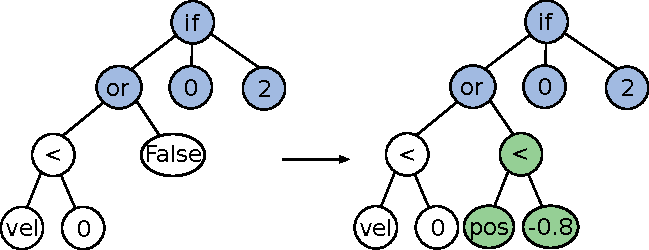
\includegraphics[width=0.75\linewidth]{../img/inkscape/fix_nodes_mutation.pdf}
\end{frame}









\section{Explainable AI} %%%%%%%%%%%%%%%%%%%%%%%%%%%%%%%%%%%%%%%%%%%%%%%%%%%%%%%%%%%%%%%%%%%%%%%%%%%%%%%%%%%

\begin{frame}{Explainable AI}
 \begin{columns}
  \column{0.5\textwidth}
  Interpretability
   \begin{itemize}
	\item How is the problem formulation incomplete?
	\item Level of evaluation? 
	\item Task-related factors? (e.g. global/local, incompleteness, user expertise, time)
	\item Method-related factors (e.g. form/number/compositionality of cognitive chunks, monotonicity, uncertainty)
   \end{itemize}
  \column{0.5\textwidth}
   \includegraphics[width=0.85\textwidth]{img/lrp_example.pdf}
   Example: Layerwise Relevance Propagation
   \begin{itemize}
	\item Relevance feedback in an NN
	\item Marks the decisive pixels
	\item Local interpretability
   \end{itemize}
 \end{columns}
\end{frame}

\begin{frame}{Explainability Gap}
\centering
\includegraphics[height=0.89\textheight]{../img/inkscape/explainability_gap2_minimal_beamer.pdf}
\end{frame}










\section{Implementation} %%%%%%%%%%%%%%%%%%%%%%%%%%%%%%%%%%%%%%%%%%%%%%%%%%%%%%%%%%%%%%%%%%%%%%%%%%%%%%%%%

\begin{frame}{Tree Edit distance}
%
\includegraphics[height=0.89\textheight]{img/concept.png}  % aka 76m
\centering
\includegraphics[height=0.75\textheight]{../img/inkscape/ted_operators.pdf}
\end{frame}

\begin{frame}{Fixed Core}
 \begin{figure}[th]
  \centering{}
  \plforest{[{$\text{if-then-else}$},fixnode[{$<$}[{vel}][{$0$}]][{$0$},fixnode][{$2$},fixnode]]}  
  \caption{The expert might want to only change the condition of the if-statement,
as he can then better understand the distinction. In his start-up
program, he would specify the nodes marked in dark blue as fixed so
that they are not affected by the GP process.}
 \end{figure}
\end{frame}

\begin{frame}{Tight tree nodes}
\centering
\begin{figure}[tph]
\begin{centering}
\plforest{[if-then-else[$<$[vel][$0$]][$0$][$2$]]}\hspace{8mm}\plforest{[{$+$}[abs[pos]][{$\cdot$}[{$174.162$}][{vel}]]]} \hspace{8mm}\plforest{[{$x^y$}[vel][{$-5.0$}]]} 
\par\end{centering}
\caption{Three formulas with completely different approaches that achieve almost
identical results.}
\end{figure}
\end{frame}

\begin{frame}{Visualization: Tight Tree Nodes}
\centering
\begin{figure}[th]
\begin{centering}
\begin{tabular}{ccc}
\plforest{[{if-then-else}[{$<$}[{vel}][{$0$}]][{$\div$}[{pos}][{$-1.834$}]][{$2.197$}]]} &  & \plforest{[{if-then-else}[{$<$}[{vel}][{$0$}]][{{${\frac{\text{pos}}{-1.834}}$}}][{$2.197$}]]}\tabularnewline
\end{tabular}
\par\end{centering}
\caption{Automatic visualization of a tree with all nodes and as a tight version.}
\end{figure}
\end{frame}

\begin{frame}
 \frametitle{Mountain car policies}
 \begin{columns}
  \column{0.30\textwidth}
   \includegraphics[height=0.4\textheight]{img/mtc/decisions-sarsa_agent_75.pdf}
   \includegraphics[height=0.4\textheight]{img/mtc/decisions-XiaoPresetAgent.png}
  \column{0.30\textwidth}
   
\includegraphics[height=0.4\textheight]{img/mtc/decisions-sarsa_agent_200.pdf}
   \includegraphics[height=0.4\textheight]{img/mtc/decisions-Good_Expert.png}
  \column{0.4\textwidth}
   Different policies
   \begin{itemize}
 	  \item Neural networks
 	  \item Mathematical formula
 	  \item Domain expert (human)
   \end{itemize}
 \end{columns}
\end{frame}









%%%%%%%%%%%%%%%%%%%%%%%%%%%%%%%%%%%%%%%%%%%%%%%%%%%%%%%%%%%%%%%%%%%%%%%%%%%%%%%%%%%%%%%%%%%%%%%%%%%%%%%
\section{Evaluation}

\begin{frame}{Industrial Benchmark Data}
\begin{table}[tph]
\noindent \centering{}%
\begin{tabular}{>{\centering}p{1.8cm}>{\centering}p{1.6cm}>{\centering}p{1.5cm}>{\centering}p{1.5cm}>{\centering}p{1.5cm}>{\centering}p{1.5cm}>{\centering}p{1.5cm}}
\toprule 
 & setpoint & velocity & gain & shift & fatigue & consumption\tabularnewline
\midrule
Acronym & p & v & g & h & f & c\tabularnewline
Description & external driver, constant &  &  &  & reward & reward\tabularnewline
action & - & $\pm1$ & $\pm1$ & $\pm1$ & - & -\tabularnewline
Min/Max & $[10,100]$ & $[0,100]$ & $[0,100]$ & $[0,100]$ & $[0,100]$ & $[0,100]$\tabularnewline
\midrule 
Mean & 55 & 48.75 & 50.53 & 49.45 & 37.51 & 166.33\tabularnewline
Deviation & 28.72 & 12.31 & 29.91 & 29.22 & 31.17 & 139.44\tabularnewline
retrospective &  & 10 & 10 & 10 & 10 & 10\tabularnewline
\bottomrule
\end{tabular}
\end{table}
\end{frame}






%%%%%%%%%%%%%%%%%%%%%%%%%%%%%%%%%%%%%%%%%%%%%%%%%%%%%%%%%%%%%%%%%%%%%%%%%%%%%%%%%%%%%%%%%%%%%%%%%%%%%%%
\section{Mountain Car}

\begin{frame}{Mountain Car - Simple Agent Improvements}
 \begin{columns}
  \column{0.30\textwidth}
   \begin{tabular}{cc}
    \multicolumn{2}{c}{TED=6}\tabularnewline
    $\ensuremath{\text{MSE=}0.12}$ & $R=-106.4$\tabularnewline
   \end{tabular}
   \includegraphics[height=3cm]{../../benchmarks/slurm_runs/MTC200_MAE_simpleFix/sfehs_eval/space-6} 
  \column{0.7\textwidth}
   \plforest{[$\text{if-then-else}$,fixnode[$<$,samenode[vel,samenode][$-0.014 \cdot \text{pos}^2$\\$-0.243$]][$0$,fixnode][$2$,fixnode]]} 
 \end{columns}
\end{frame}

\begin{frame}{Mountain car policies}
  Simple expert policy:\\
   ``Accelerating towards the current direction''
 \begin{columns}
  \column{0.5\textwidth}
   \includegraphics[height=0.4\textheight]{img/mtc/decisions-SimpleAgent.pdf}
  \column{0.5\textwidth}
   Potential improvements:
   \begin{itemize}
 	\item Reverse early
 	\item Are two or three swings necessary?
 	\item Always accelerate
   \end{itemize}
 \end{columns}
\end{frame}

\begin{frame}{Mountain Car - Simple Program Improvements}
 \begin{columns}
  \column{0.30\textwidth}
   \begin{tabular}{cc}
    \multicolumn{2}{c}{TED=11}\tabularnewline
    $\ensuremath{\text{MSE=}0.09}$ & $R=-100.6$\tabularnewline
   \end{tabular}
   \includegraphics[height=3cm]{../../benchmarks/slurm_runs/MTC200_MAE_simpleFix/sfehs_eval/space-11}
  \column{0.7\textwidth}
   \plforest{[$\text{if-then-else}$,fixnode[$<$,samenode[vel,samenode][$\text{if-then-else}$[$<$[vel][$-0.008$]][$0$][$\text{pos} \cdot {{\text{pos}^2}^2}$\\$-0.047$]]][$0$,fixnode][$2$,fixnode]]} 
 \end{columns}
\end{frame}

\begin{frame}{Mountain Car - Simple Program Improvements}
 \begin{columns}
  \column{0.30\textwidth}
   \begin{tabular}{cc}
    \multicolumn{2}{c}{TED=20}\tabularnewline
    $\text{MSE}=0.05$ & $R=-98.1$\tabularnewline
   \end{tabular}
   \includegraphics[height=3cm]{../../benchmarks/slurm_runs/MTC200_MAE_simpleFix/sfehs_eval/space-20}
  \column{0.7\textwidth}
   \plforest{[$\text{if-then-else}$,fixnode[$<$,samenode[vel][$\text{if-then-else}$[$<$,samenode[vel,samenode][$-0.01$\\$ \cdot {\text{pos}^2}^2$]][$1.03$][[$\text{pos} -0.03$\\$-0.73 \cdot {{\text{pos}^2}^2}$]]]][$0$,fixnode][$2$,fixnode]]} 
 \end{columns}
\end{frame}

\begin{frame}{Mountain Car - Complex Program}
 \begin{columns}
  \column{0.30\textwidth}
   \begin{tabular}{cc}
    \multicolumn{2}{c}{TED=8}\tabularnewline
    $\text{MSE}=0.07$ & $R=-98.2$\tabularnewline
   \end{tabular}
   \includegraphics[height=3cm]{../../benchmarks/slurm_runs3_easy/MTC200_MSE_simonBestFix2/sfehs_eval/space-22}
  \column{0.7\textwidth}
   \includegraphics[width=0.95\textwidth]{img/MC_ifex_8.pdf}
 \end{columns}
 %\includegraphics[height=3cm]{../../benchmarks/slurm_runs3_easy/MTC200_MSE_simonBestFix2/sfehs_eval/space-22}\\
 %\plforest{[$\text{if-then-else}$,fixnode[$\lor$,fixnode[$\land$,fixnode[$\text{pos}<$\\$-0.35$][$0.013$\\$<\text{vel}$]][$\land$,fixnode[$\text{pos}-$\\$(10.4 \cdot \text{vel})$\\$<-0.82$][$-\text{vel}<$\\$0.015$]]][$2$,fixnode][$\text{if-then-else}$,fixnode[$\land$,fixnode[$\text{vel}<$\\$0.02$][$\land$,fixnode[$>$[$\text{if-then-else}$[$\text{pos}>-0.38$][pos][$\text{pos}-9.9 \cdot \text{vel}$]][$-0.46$]][$\text{pos}<-0.05$]]][$0$,fixnode][$\text{if-then-else}$,fixnode[$\text{vel}<0$,fixnode][$0$,fixnode][$2$,fixnode]]]]}
\end{frame}

\begin{frame}{Mountain Car - Parabolic Formula}
\centering
\includegraphics[height=0.85\textheight]{img/genetic_extensions_2.pdf} 
\end{frame}





%%%%%%%%%%%%%%%%%%%%%%%%%%%%%%%%%%%%%%%%%%%%%%%%%%%%%%%%%%%%%%%%%%%%%%%%%%%%%%%%%%%%%%%%%%%%%%%%%%%%%%%
\section{Industrial Benchmark}

\begin{frame}{Industrial Benchmark - Results ''s3m``}
 \centering
 \includegraphics[height=0.85\textheight]{../img/inkscape/ib_vis/ib_pp_1.pdf}
\end{frame}

\begin{frame}{''s3m`` Industrial Benchmark - Results}
 \centering
 \includegraphics[height=0.85\textheight]{../img/inkscape/ib_vis/ib_pp_2.pdf}
\end{frame}

\begin{frame}{Industrial Benchmark - Results ''s3m``}
 \centering
 \includegraphics[height=0.85\textheight]{../img/inkscape/ib_vis/ib_pp_3.pdf}
\end{frame}

\begin{frame}{Industrial Benchmark - Results ''s3m``}
 \centering
 \begin{figure}[tph]
  \includegraphics[height=5cm]{../../benchmarks/slurm_runs/IB_MSE_s3m/pareto_combined.pdf}\includegraphics[height=5cm]{../../benchmarks/slurm_runs/IB_MSE_s3m/regression_all.pdf}
  \caption{\label{fig:ib-plots} The improvements of the start policy improve
the real performance without bad outliers. As the IB requires merging
multiple Pareto candidates, it is good advice to discard the first
combinations.}
 \end{figure}
\end{frame}




%%%%%%%%%%%%%%%%%%%%%%%%%%%%%%%%%%%%%%%%%%%%%%%%%%%%%%%%%%%%%%%%%%%%%%%%%%%%%%%%%%%%%%%%%%%%%%%%%%%%%%%
\section{Discussion}

\begin{frame}{Results Mountain Car vs. Industrial Benchmark}
 \centering
 \begin{figure}[tph]
 \includegraphics[height=5cm]{../../benchmarks/slurm_runs/MTC200_MSE_scratch/histograms/acthist_25.pdf}\includegraphics[height=5cm]{../../benchmarks/slurm_runs2/IB_MSE_scratch/IB_MSE_scratch_0/histograms/acthist_29.pdf}
\caption{\label{fig:Histograms-mc-ib} Histograms presenting the deviation
from the black box action in the MC (left) and the IB (right), both
regarding the best available regular GP agent (MSE). MC agents have
a very high success rate, while the best IB agent have lumps of failure
on both sides.}
\end{figure}
\end{frame}






%%%%%%%%%%%%%%%%%%%%%%%%%%%%%%%%%%%%%%%%%%%%%%%%%%%%%%%%%%%%%%%%%%%%%%%%%%%%%%%%%%%%%%%%%%%%%%%%%%%%%%%
\section{Future work}

\begin{frame}
\centering
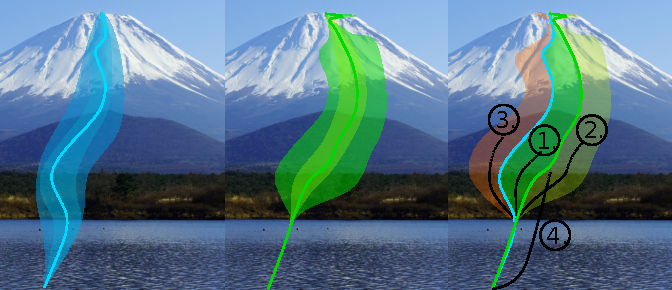
\includegraphics[width=0.9\linewidth]{../img/inkscape/explorative_regression_hill.pdf}
\end{frame}



\end{document}











